% This is part of Un soupçon de physique, sans être agressif pour autant
% Copyright (C) 2006-2009,2016
%   Laurent Claessens
% See the file fdl-1.3.txt for copying conditions.


\subsection{Loi de Snell-Descartes et vitesse de la lumière}   \label{SubsecSnellVitesse}
%-----------------------------------------------------------

\paragraph{Avertissement}
La preuve apportée ici à la loi de Snell-Descartes utilise le fait que la lumière se comporte comme une onde. La notion de front d'onde sera utilisée. Le niveau est donc un peu plus élevé que d'habitude.

\paragraph{}

Le phénomène de réfraction est dû à une différence de vitesse de propagation de la lumière entre deux milieux. Prenons l'exemple de l'air et de l'eau. Dans l'air, la lumière parcours environ \unit{300\,000}{\kilo\meter\per\second}, tandis que dans l'eau cette vitesse n'est que de \unit{225\,000}{\kilo\meter\per\second}. 

Considérons un paquet de rayons de lunes parallèles qui arrivent à la surface d'un étang par une belle nuit étoilée. Tant que la lumière ne touche pas du tout l'eau, tous les rayons avancent ensemble, au moment où des rayons commencent à pénétrer dans l'eau, les choses commencent à se compliquer. Durant le temps entre le moment où le premier rayon entre dans l'eau et le moment où les deux autres y parviennent, le premier rayon avance moins vite que les deux suivants. On voit alors tout de suite que le tout ne va plus avancer en un bloc, mais se déformer.

Il est donc clair qu'il va se passer quelque chose. Pouvons-nous voir plus précisément ce qui va se passer ?

\begin{exercice}
Le rayon de la Terre vaut \unit{6500}{\kilo\meter} à l'équateur. Combien de tours de la Terre la lumière peut-elle faire en une seconde. Le Soleil se trouve à \unit{149\,600\,000}{\kilo\meter} de la Terre. Combien de temps mets la lumière solaire pour arriver jusqu'à nous ? 

Mars se trouve à \unit{227\,900\,000}{\kilo\meter} du Soleil. Quelle est la distance minimale que l'on peut espérer trouver entre la Terre et le Soleil ? Combien de temps il faut à la lumière pour aller de la Terre à Mars dans ces conditions ? Cela incite à la plus grande prudence quand on télécommande des robots sur Mars depuis la Terre, et peut poser des problèmes pratiques quant à l'organisation d'un tournois d'échecs interplanétaire.
\end{exercice}

\subsubsection{Physique de la réfraction}
%-------------------------------------

\begin{figure}[ht]
\centering

\subfigure[Le trait bleu pointillé représente le trajet que le rayon $B$ doit encore parcourir avant d'arriver sur l'interface au moment où le rayon $B$ vient d'y arriver]{%
\label{lepremier}
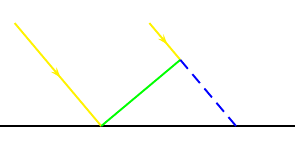
\includegraphics{fig3832_1.png}
}
%
\subfigure[Où le rayon $A$ a-t-il pu aller durant ce temps ?]{%
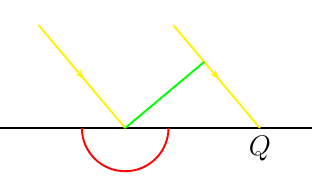
\includegraphics{fig3832_2.png}
\label{ledeux}
}
%
\subfigure[Pas correct]{%
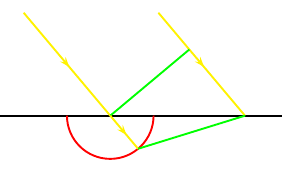
\includegraphics{fig3832_3.png}
\label{lepasbon}
} 
%
\subfigure[Correct]{%
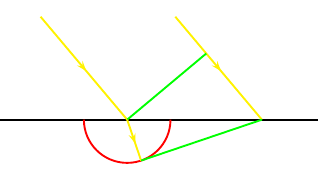
\includegraphics{fig3832_4.png}
\label{lebon}
}

\caption{Réfraction : étude de la physique du phénomène.}\label{fig_refr_phyz}
\end{figure}

Étudions en détail les trajets suivis par deux rayons lumineux parallèles $A$ et $B$ qui arrivent sur un interface, voir les figures \ref{fig_refr_phyz}. Disons que leur vitesse vaut $v_{1}$ dans le premier milieu et $v_{2}$ dans le second. On suppose $v_{2}<v_{1}$. 

La figure \ref{lepremier} montre la situation au moment où le rayon $A$ arrive à l'interface : à ce moment il va se passer quelque chose pour lui, tandis que $B$ doit encore parcourir le trajet bleu avant d'avoir à se soucier de quoi que ce soit. Le front d'onde est dessiné en vert et est, comme il se doit, perpendiculaire aux deux rayons en même temps.

Un peu plus tard, le rayon $B$ arrive à l'interface, c'est la figure \ref{ledeux}. Durant le temps que le rayon $B$ a mit pour arriver là (c'est à dire le temps pour lui de parcourir le trajet bleu de la figure \ref{lepremier}), le rayon $A$ a pu parcourir dans le second milieu une distance $v_{2}/v_{1}$ fois moins longue. Ce rayon est donc quelque part sur le demi-cercle rouge dont le rayon vaut $v_{2}/v_{1}$ fois la longueur du trajet bleu.

Le fait physique qui permet de déterminer à quel endroit du cercle rouge se trouve le rayon $A$ est le suivant : le front d'onde doit être perpendiculaire au rayon. Il faut donc qu'un segment allant du bout du rayon $A$ vers le point $Q$ (qui est le bout du rayon $B$) soit perpendiculaire au rayon $A$. En d'autres termes, il faut trouver la tangente au cercle rouge passant par le point $Q$\footnote{Ici, on a utilisé un peu de géométrie : une droite qui coupe un cercle en \emph{un seul} point $R$ est tangente au cercle si et seulement si elle est perpendiculaire au rayon $\overrightarrow{OR}$.}.

Sur la figure \ref{lepasbon}, nous avons fait comme si le rayon $A$ n'était pas dévié. On voir immédiatement que le front d'onde vert n'est pas perpendiculaire au rayon. Ce point n'est pas le bon. Attention : nous ne demandons pas que les deux fronts d'ondes dessinés soient parallèles.

Sur la figure \ref{lebon}, nous avons soigneusement pris le point de tangence comme destination du rayon $A$.


Le travail à présent est de déterminer exactement la déviation en fonction de $v_{1}$ et de $v_{2}$.

\subsubsection{Petit retour en arrière : la réflexion}
%---------------------------------------------------

Maintenant qu'on a compris comment les rayons se comportent lors d'un changement de milieu, on peut expliquer la loi des angles égaux lors de la réflexion. En effet entre la figure \ref{lepremier} et \ref{ledeux}, nous avons supposé que le rayon $A$ allait continuer à l'intérieur du second milieu. Mais que se passerait-t-il si au lieu de cela, il retournait en arrière ? Pour la figure \ref{fig_refl_pm}, nous reprenons la situation de la figure \ref{fig_refr_phyz}, sauf que cette fois nous traçons le cercle rouge vers le haut plutôt que vers le bas.

Nous reprenons l'argument de la tangente pour dessiner la figure \ref{latroisrefl}.

\begin{figure}[ht]
\centering

\subfigure[Le trait bleu pointillé représente le trajet que le rayon $B$ doit encore parcourir avant d'arriver sur l'interface au moment où le rayon $B$ vient d'y arriver]{%
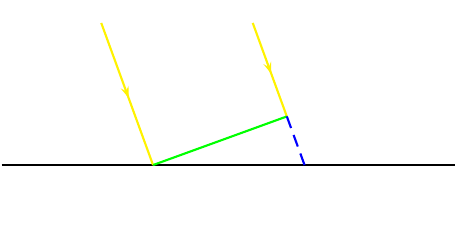
\includegraphics{fig22788_1.png}
\label{lepremierrefl}
}
%
\subfigure[Le rayon a pu se réfléchir en allant vers un des points du cercle rouge. Mais cette fois, le cercle a un rayon de la même taille que le trajet bleu de la figure \ref{lepremierrefl} parce que la réflexion se fait dans le même milieu que l'incidence]{%
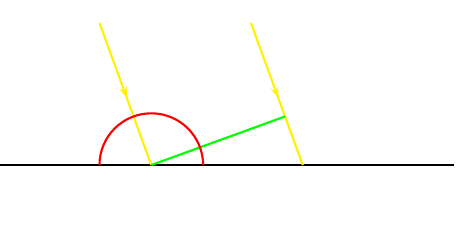
\includegraphics{fig22788_2.png}
\label{lesecondrefl}
}
%
\subfigure[Le rayon $A$ se réfléchit de telle façon à ce que le front d'onde soit tangent au cercle rouge]{%
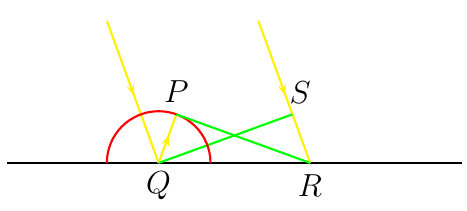
\includegraphics{fig22788_3.png}
\label{latroisrefl}
}
%
\caption{Réflexion : étude de la physique du phénomène.}\label{fig_refl_pm}
\end{figure}

\begin{exercice}
Prouvez que les triangles $PQR$ et $SRQ$ de la figure \ref{latroisrefl} sont identiques, et déduisez-en les relations voulues, c'est à dire essentiellement que les angles $\widehat{PQR}$ et $\widehat{SRQ}$ sont égaux.

Pour cela, n'hésitez pas à utiliser les faits que l'angle $\widehat{QSR}$ est droit, et que les deux rayons lumineux sont parallèles dans le premier milieu.
\end{exercice}

\subsubsection{Résolution géométrique de la réfraction}
%-----------------------------------------------------

La figure \ref{figRefracGeom} montre la géométrie du problème de réfraction. Le but est de trouver l'angle $\beta$ de réfraction (celui entre le rayon réfracté et la normale) en fonction de l'angle d'incidence $\alpha$ (entre le rayon incident et la normale), en sachant que 
\begin{equation}  \label{eq_rappvitlong}
  \| AC \|=\frac{ v_{2} }{ v_{1} }\| DB \|.
\end{equation}


Nous désignons par $\alpha'$ et $\beta'$ les angles $90-\alpha$ et $90-\beta$, et nous laissons comme exercice le soin de comprendre pourquoi les angles indiqués sont corrects (pensez que dans un triangle rectangle, la somme des deux angles non droit vaut $90$ degrés). 

En regardant attentivement les triangles rectangles $ADB$ et $ACB$, on trouve que 
\[
  \cos\beta'=\frac{ \| AC\| }{ \| AB \| }\text{ et }
  \cos\alpha'=\frac{ \| BD \| }{ \| AB \| },
\]
et donc
\begin{equation}   \label{EqCossinVV}
\frac{ \cos\beta' }{ \cos\alpha' }=\frac{ \sin\beta }{ \sin\alpha }=\frac{ \| AC \| }{ \| BD \| }=\frac{ v_{2} }{ v_{1} }.
\end{equation}
Dans cette ligne, nous avons d'abord utilisé l'égalité trigonométrique comme quoi $\cos(90-x)=\sin(x)$, et ensuite l'hypothèse \eqref{eq_rappvitlong}. 

Une faute que l'on pourrait commettre est la suivante : étant donné que le front d'onde est toujours perpendiculaire au rayon, il faut que $\overrightarrow{CB}$ soit perpendiculaire à $\overrightarrow{DB}$, de sorte que $\alpha'+\beta=90$. Ce n'est pas le cas parce qu'en fait le front d'onde $CB$ dessiné n'est valable qu'à l'intérieur du milieu du bas, tandis que le rayon $DB$ est encore dans le premier milieu.

\begin{figure}
    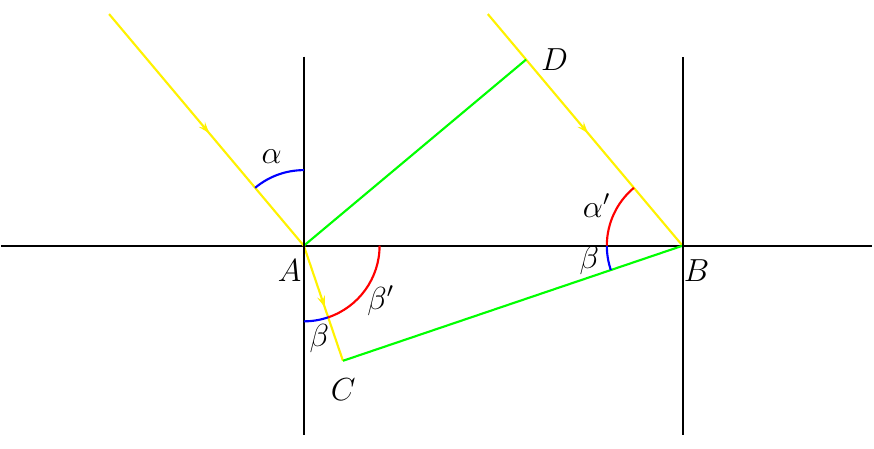
\includegraphics{fig1617_1.png}
\caption{La réfraction}\label{figRefracGeom}
\end{figure}

\subsubsection{Les indices absolus}
%//////////////////////////////////

Reprenons les parties importantes de l'équation \eqref{EqCossinVV}, en changeant de notations (je te laisse deviner ce qui vaut quoi) :
\begin{equation}
\frac{ \sin\hat\imath }{ \sin\hat r }=\frac{ v_{1} }{ v_{2} }.
\end{equation}
Si on désigne par $c$ la vitesse de la lumière dans le vide\footnote{Environ \unit{3\cdot\power{10}{8}}{\meter\per\second}.}, et qu'on définit
\[ 
 n_{1}=\frac{ c }{ v_{1} },\quad n_{2}=\frac{ c }{ v_{2} },
\]
on peut écrire
\begin{equation}   \label{EqFormSnell}
\frac{ \sin\hat\imath }{ \sin\hat r }=\frac{ n_{2} }{ n_{1} }.
\end{equation}
Les nombres $n_{1}$ et $n_{2}$ sont appelée les \defe{indices absolus}{} des milieux $1$ et $2$. En comparant avec l'équation \eqref{EqSinNDeuxUn}, on trouve que les indices relatifs sont donnés par le indices absolus par la formule
\[ 
  n_{2/1}=\frac{ n_{2} }{ n_{1} }.
\]

\subsection{Réfringence}
%------------------------

Si $n_{2/1}>1$, on a que $\sin\hat\imath>\sin\hat r$, et donc $\hat\imath>\hat r$. Ce cas est illustré sur la figure \ref{SubFigRefrUn}; le cas inverse est donné à la figure \ref{SubFigRefrDeux}. Par exemple, l'eau est plus réfringente que l'air.

 Les deux règles que l'on déduit sont :
\begin{enumerate}
\item Un rayon lumineux passant d'un milieu moins réfringent dans un milieu plus réfringent se rapproche de la normale.
\item Un rayon lumineux passant d'un milieu plus réfringent dans un milieu moins réfringent s'écarte de la normale.
\end{enumerate}

\begin{figure}[ht]
\centering
\subfigure[Le milieu $1$ est plus réfringent que le milieu $2$.]{%
    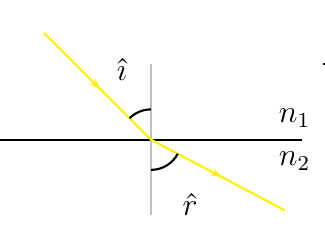
\includegraphics{fig1848_1.png}
\label{SubFigRefrUn}
}
%
\subfigure[Le milieu $2$ est plus réfringent que le milieu $1$.]{%
    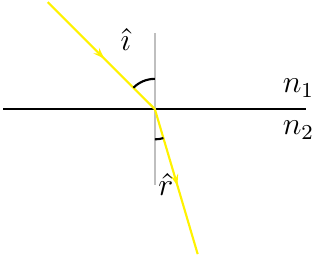
\includegraphics{fig1848_2.png}
\label{SubFigRefrDeux}
}
\caption{Second milieu plus ou moins réfringent que le premier.}\label{FigRefringence}
\end{figure}

\subsection{Construction du rayon réfracté}
%------------------------------------------

Nous nous donnons comme but de construire (par dessin) le rayon réfracté lorsqu'on connaît l'indice de réfraction et le rayon incident. Nous nous donnons la situation de la figure \ref{SubFigConstructionUn} où un rayon $AO$ arrive à la surface de séparation (la droite $XY$) entre de l'air et de l'eau ($n_{\text{eau/air}}=4/3$).

D'abord nous faisons un choix d'unité sur l'axe $XY$, et on place $C$ à $4$ unités de $B$. De là, on élève la perpendiculaire à $XY$ qui intersecte $AO$ au point $A'$, et on trace le cercle de rayon $\| OA' \|$ de centre $O$. Cela nous amène à la figure \ref{SubFigConstructionDeux}.

Maintenant on place le point $D$ à $3$ unités de $O$, et on trace la perpendiculaire qui intersecte le cercle en $E$. Le rayon recherché est $OE$, ce qui nous amène à \ref{SubFigConstructionTrois}. En effet, nous avons par construction que $\| BA' \|=\| BE \|$ (parce que $A'$ et $E$ sont sur le même cercle), et donc
\[ 
  \frac{ 4 }{ 3 }=\frac{ \| BC \| }{ \| BD \| }=\frac{ \| BC \|\,/\,\| BA' \| }{ \| BD \|\,/\,\| BE \| }=\frac{ \sin\hat\imath }{ \sin\hat r }.
\]

\begin{figure}[ht]
\centering
\subfigure[Comment construire le rayon réfracté dans cette situation ?]{%
    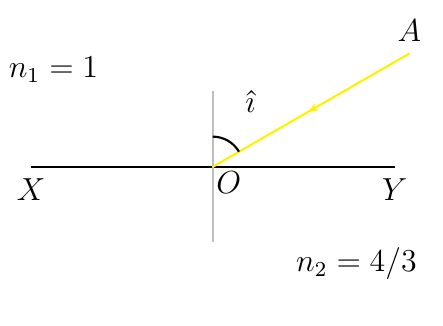
\includegraphics{fig30125_1.png}
\label{SubFigConstructionUn}
}
%
\subfigure[Une première étape de la construction]{%
    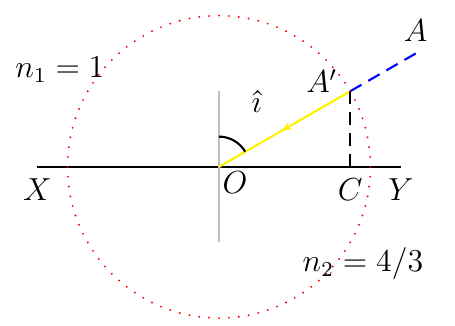
\includegraphics{fig30125_2.png}
\label{SubFigConstructionDeux}
}
\subfigure[La solution]{%
    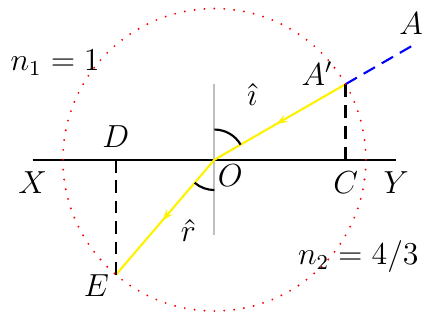
\includegraphics{fig30125_3.png}
\label{SubFigConstructionTrois}
}
\caption{Construction géométrique d'un rayon réfracté.}\label{FigConstruction}
\end{figure}

\subsection{Angle limite de réfraction}
%--------------------------------------

Lors du passage de l'air vers l'eau, la déviation du rayon réfracté augmente avec l'angle d'incidence, voir figure \ref{FigRasants}. La déviation est maximale quand $\hat\imath=\unit{90}{\degree}$, dans ce cas, on a 
\[ 
  \frac{ \sin\unit{90}{\degree} }{ \sin\hat r_{l} }=\frac{ 4 }{ 3 },
\]
et donc $\hat r_{l}=\unit{48}{\degree}\unit{36}{\arcminute}$. Il n'est pas possible de faire dévier un rayon plus fort que cet angle en passant de l'air à l'eau.

En général, à chaque fois que l'on passe d'un milieu moins réfringent vers un milieu plus réfringent, il existe un angle limite de réfraction donné par
\[ 
  \sin\hat r_{\text{max}}=\frac{1}{ n_{2/1} },
\]
voir la figure \ref{FigRasants}. 

\begin{figure}[ht]
\centering
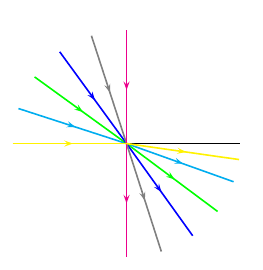
\includegraphics{fig20947_1.png}
\caption{Comment des rayons incidents de plus en plus rasants se réfractent.} \label{FigRasants}
\end{figure}


\subsection{Réflexion totale}
%----------------------------

Regardons un peu les conditions d'existence pour $\hat r$ dans la formule \eqref{EqFormSnell} que l'on écrit sous la forme
\begin{equation} \label{EqVarharrsinimath}
  \sin\hat r=\frac{ \sin\hat\imath }{ n_{2/1} }.
\end{equation}
Le sinus d'un angle ne peut pas être plus grand que $1$, donc si on veut que cette formule définisse correctement $\hat r$, il faut que 
\[
\sin\hat\imath\leq n_{2/1}.
\]
Étant donné que $\sin\hat\imath\in[-1,1]$, on ne risque de faillir à satisfaire cette condition uniquement lorsque $n_{2/1}<1$ (on a toujours que $n_{2/1}>0$). Les problèmes ne peuvent donc arriver que lorsque le rayon passe d'un milieu plus réfringent à un moins réfringent. Par exemple le passage de l'eau à l'air.

Au cas où $\sin\hat r>1$, on ne peut pas trouver de $\hat r$, et le phénomène physique correspondant est qu'il n'y a aucun rayon réfracté : toute la lumière est réfléchie, voir la figure \ref{FigReflTot}.

\begin{exercice}
Si vous voulez expérimenter la réflexion totale à la piscine, est-ce qu'il vous faut une lampe de poche qui résiste à l'eau ? En d'autres termes, allez-vous mettre la lampe sous l'eau et regarder la lumière qui sort de l'eau, ou bien mettre la lampe en dehors de l'eau et regarder la lumière qui rentre dans l'eau ? Le phénomène va-t-il être observé quand la lampe est presque parallèle à l'eau, ou bien au contraire quand elle est presque perpendiculaire ?
\end{exercice}

\begin{figure}[ht]
\centering
\subfigure[Un rayon sort de l'eau avec un angle relativement petit par rapport à la normale.]{%
    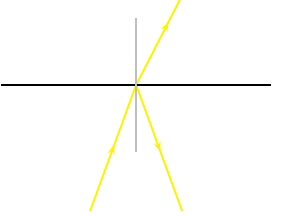
\includegraphics{fig3707_1.png}
}						% Cette fermeture est celle de la sous-figure.
%
\subfigure[Le rayon arrive avec un angle maximum, le rayon réfracté existe encore mais rase l'interface. Bonne chance pour réaliser ça dans une piscine ou à la mer, à cause des vagues !]{%
    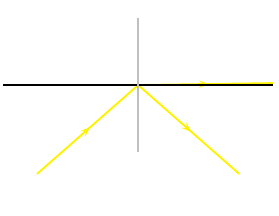
\includegraphics{fig3707_2.png}
}
%
\subfigure[Maintenant l'angle est trop grand, il n'y a plus de rayon réfracté.]{%
    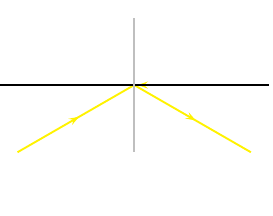
\includegraphics{fig3707_3.png}
}
\caption{Phénomène de réflexion totale}\label{FigReflTot}
\end{figure}

L'équation \eqref{EqVarharrsinimath} donne $\hat r$ par la formule  \label{PgExpCErefrtot}
\[ 
  \hat r=\arcsin\Big( \frac{ \sin\hat\imath }{ n_{2/1} } \Big).
\]
Il est remarquable de comprendre que le phénomène de réflexion totale est une manifestation physique tout à fait palpable de la condition d'existence $| x |\leq1$ pour la fonction $x\mapsto\arcsin x$ que tu auras vue dans un cours de math que tu croyais être complètement inutile et abstrait. Eh bien non : cette condition d'existence a un contenu physique, la nature la respecte. C'est un fait très général en science : il semble que la nature s'amuse à suivre des lois mathématiques de façon très rigoureuse. 

\subsection{Exercices}
%---------------------

\Exo{108}
\Exo{104} 
\Exo{105} 
\Exo{106} 
